\section[Bachelor-Studiengang Physik]{Bachelor-Studiengang Physik\\(und Studienrichtung Scientific Instrumentation)}
\begin{multicols}{2}
\begin{quote}
	\textit{Die Wissenschaft ist nichts als das Abbild der Wahrheit.}
	
	\hfill--- Francis Bacon
\end{quote}
Unter "Ziel des Studiums" steht in der Prüfungsordnung der erste Satz:
\begin{quote}
	\textit{"Das Bachelor-Studium ist ein grundständiges wissenschaftliches Studium, das zu einem ersten berufsqualifizierenden Abschluss führt."}
\end{quote}
Wie dies hier in Münster erreicht wird, wird in diesem Artikel vorgestellt.
Da sich die Prüfungsordnung bisher jedes Jahr wieder geändert hat, gehe ich davon aus, dass die Version, über die ich hier schreibe (Bachelor-Prüfungsordnung vom Sommersemester 2015), schon bald nicht mehr aktuell sein könnte.

Des Weiteren sei direkt vorweggenommen, dass der Bachelor in der Regel \emph{keinen} berufsqualifizierenden Abschluss darstellt, sondern ein Physiker häufig erst ab einem Master-Abschluss auch von der Wirtschaft akzeptiert wird.

\subsection{Modularisierung}
Das Studium gliedert sich in Module.
Ein Modul ist eine inhaltlich zusammenhängende Einheit aus mehreren Studienleistungen wie Vorlesung, Übung, Seminar, Praktikum oder Ähnlichem.
Nach dem European Credit Transfer System~(ECTS) werden Module mit Leistungspunkten (LP; manchmal auch Credit~Points, CP) gewichtet.
Ein LP entspricht dabei einem Studienaufwand von \SI{30}{\hour}, wobei hier Präsenz- und Selbststudium gemeint ist.

Der Bachelor ist bei \SI{180}{\LP} erreicht, wobei die zu belegenden Module kaum Wahlfreiheit lassen.
Einzig das Nebenfach (Modul "Fachübergreifende Studien"), die Entscheidung über den favorisierten Abschluss und die Wahl vereinzelter Kurse wird dem Studierenden überlassen.
Daher lässt sich der Studienverlaufsplan für alle recht genau angeben.
Aufgrund der bisher genannten Probleme ist dieser jedoch mit Vorsicht zu genießen, da die Prüfungsordnung immer mal wieder angepasst wird, um das Studium und die Studienorganisation wieder zu vereinfachen.
Über derartige Wechsel wird euch aber auch die Fachschaft informieren.

\subsection{Studienverlauf und Inhalte}
\subsubsection{Erstes Studienjahr}
"Physik~I" ist eine Vorlesung mit Übung.
Hier werden 6~Semesterwochenstunden (SWS) Vorlesung besucht und es finden 4~SWS Übung statt, wobei in den Übungen Anwesenheitspflicht besteht.
Die wöchentlichen Übungszettel zu dieser Vorlesung müssen bearbeitet werden und bei einer erfolgreichen Bearbeitung von \SI{50}{\percent} der Übungsaufgaben wird man zur Modulabschlussprüfung (dreistündige Klausur) zugelassen.
In diesem Modul werden grundlegende Methoden der Physik sowie die klassische Mechanik gelehrt.
Außerdem wird in die relativistische Mechanik eingeführt.

"Mathematik für Physiker~I" ist auch eine Vorlesung (4~SWS) mit Übung (2~SWS), gehört jedoch zum Modul "Mathematische Grundlagen", welches auch die Vorlesung "Mathematik für Physiker~II" beinhaltet.
Die Klausur zu Mathe~I ist nur eine Studienleistung, kann also beliebig oft wiederholt werden und geht nicht in die Bachelor-Note ein.
Wie bei Physik~I auch müssen die Übungen besucht und bestanden werden.

\vspace{\fill}

\fibelimgtext[above right]{
	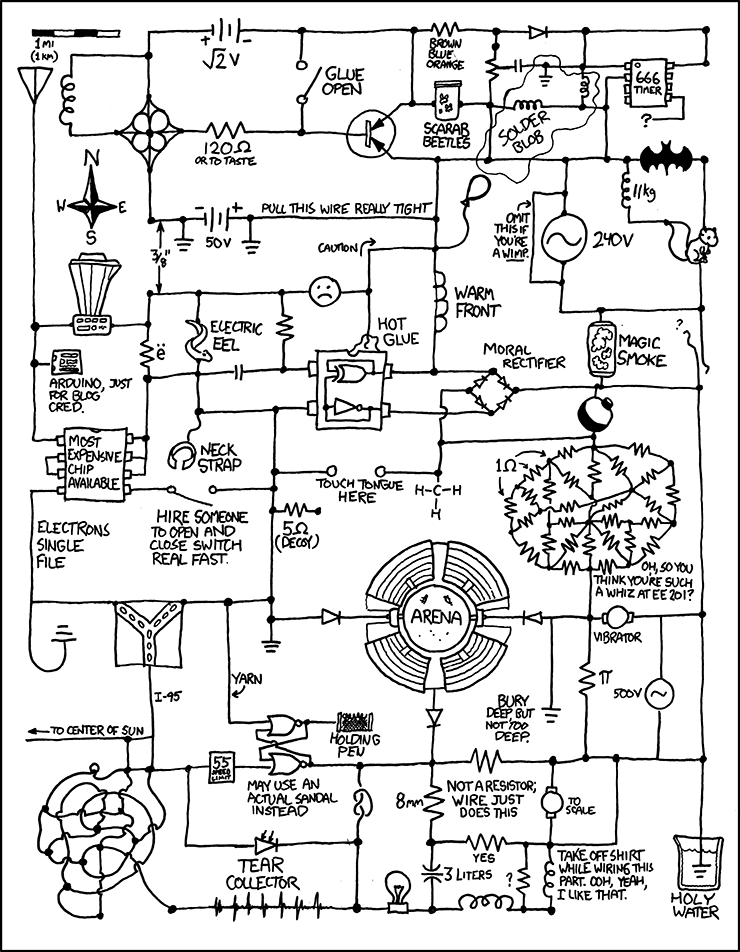
\includegraphics[width=\columnwidth]{res/xkcd/730_circuit_diagram.png}
}{\url{https://xkcd.com/730}}

% vergleiche auch Tabelle im Artikel Bachelor_Geophysik.tex
\begin{table*}
% Der Befehl \fibnl ist ein Zeilenumbruch
\let\fibnl=\par
% Länge \fibtemp ist die Breite einer Spalte in der Tabelle
% (außer Spalte mit den Semestern)
\setlength{\fibtemp}{0.195\textwidth}
% Mehrfachzeilen (horizontal) zentrieren
\renewcommand{\multirowsetup}{\centering}

\begin{tabularx}{\textwidth}{| X | *{4}{>{\centering\arraybackslash}m{\fibtemp}|}}
\hline
\textbf{Semester} & \multicolumn{4}{c|}{\textbf{Module im B.\ Sc.\ Physik}}
\\ \hline
1.\ (WS) &
	Physik~I\fibnl
	\SI{14}{\LP} (PM) &
	&
	\multirow{2}[5]{\fibtemp}{Grundlagen der Mathematik\fibnl
		\SI{16}{\LP} (PM)} &
	\multirow{3}[5]{\fibtemp}{Fachübergreifende Studien\fibnl
		\SI{18}{\LP} (WPM\textsuperscript{*})}
\\ \cline{1-3}
2.\ (SS) &
	Physik~II\fibnl
	\SI{14}{\LP} (PM) &
	&
	&
\\ \cline{1-4}
3.\ (WS) &
	Physik~III\fibnl
	\SI{14}{\LP} (PM) &
	\multirow{2}[5]{\fibtemp}[-1ex]{Experimentelle Übungen~I\fibnl
		\SI{13}{\LP} (PM)} &
	Integrationstheorie\fibnl
	\SI{8}{\LP} (PM) &
\\ \cline{1-2}\cline{4-5}
4.\ (SS) &
	Atom- und Quantenphysik\fibnl
	\SI{10}{\LP} (PM) &
	&
	\multirow{2}[5]{\fibtemp}{Computational Physics\fibnl
		\SI{9}{\LP} (PM)} &
	Messtechnik und Signalverarbeitung\fibnl
	\SI{8}{\LP} (PM)
\\ \cline{1-3}\cline{5-5}
5.\ (WS) &
	Struktur der Materie\fibnl
	\SI{14}{\LP} (PM) &
	\multirow{2}[5]{\fibtemp}[-1ex]{Experimentelle Übungen~II\fibnl
		\SI{13}{\LP} (PM)} &
	&
	\multirow{2}[5]{\fibtemp}[-1ex]{Berufsfeld-Differenzierung\fibnl
		\SI{16}{\LP} (WPM\textsuperscript{**})}
\\ \cline{1-2}\cline{4-4}
6.\ (SS) &
	Examensmodul\fibnl
	\SI{13}{\LP} (PM)	&
	&
	&
\\ \hline
\end{tabularx}

\framebox[\textwidth]{
\begin{minipage}{0.95\textwidth}
\centering
PM: Pflichtmodul; WPM: Wahlpflichtmodul

\raggedright
\textsuperscript{*}: Fachübergreifendes Modul, "das in einer sinnvollen Beziehung zum Studium der Physik steht oder der Berufsbefähigung dient"

\textsuperscript{**}:
\begin{minipage}[t]{0.95\linewidth}
	\begin{itemize}[nosep, wide]
		\item Quantentheorie und Statistische Physik (Studiengang Physik) oder
		\item Physikalische Instrumente und Messmethoden (Studienrichtung Scientific Instrumentation)
	\end{itemize}
\end{minipage}
\end{minipage}
}
\end{table*}

% \newpage statt \clearpage, damit die Tabelle nicht auf einer eigenen Seite
% landet
\newpage

Das Modul "Fachübergreifende Studien" (Nebenfach im Umfang von \SI{18}{\LP}) kann frei aus einer vorgegebenen Auswahl getroffen werden.
Diese vorgefertigten Module sind:
\begin{itemize}[parsep=0.7ex]
	\item Einführung in die Informatik
	\item Geophysik
	\item Chemie für Physiker
	\item Philosophie für Physiker
	\item Mathematik
	\item Theoretische Grundlagen der Psychologie
	\item Einführung in die Betriebswirtschaftslehre
	\item Einführung in die Volkswirtschaftslehre
	\item Spanisch für Naturwissenschaftler
	\item (Deutsch als Fremdsprache)
\end{itemize}
Man kann auch durch Absprache mit dem Studiendekan ein mit der Physik verbundenes Modul in anderen Fachbereichen zusammenstellen.

Im zweiten Semester wird "Physik~II" belegt.
Es wird eine Vorlesung (6~SWS + 2~SWS Übung) über Thermodynamik und Elektrostatik sowie eine Vorlesung "Theoretische Ergänzungen" (2~SWS + 1~SWS Übung) über analytische Mechanik gehört.

Nach jedem Studienjahr hat man durchschnittlich \SI{60}{\LP} gesammelt.
Falls bestimmte Prüfungen nicht bestanden wurden, wird in der Regel zu einem späteren Zeitpunkt im Semester eine Nachklausur angeboten.
Eine andere Möglichkeit ist es, die Prüfung ein Jahr später zu wiederholen.
Jedoch muss man nach vier nicht bestandenen Versuchen das Studium abbrechen (dies ist eine der Verschärfungen, die es im Diplomstudium nicht gab).
\subsubsection[Zweites Studienjahr]{\hspace{-1.5em}Zweites Studienjahr}
\iffalse
% \intextsep: Abstand vor/nach dem Bild bei wrapfigure
\setlength{\intextsep}{1mm}
\begin{wrapfigure}[9]{r}[5mm]{0cm}
%	\scriptsize
	\raisebox{0pt}[\dimexpr\height - 6mm\relax]{%
		\fibelimgtext[above right]{
			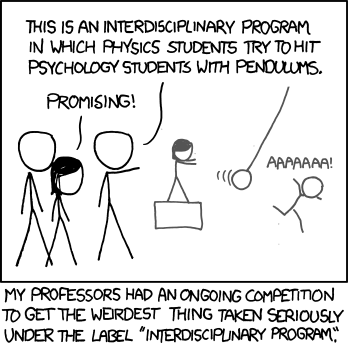
\includegraphics[width=4.7cm]{res/xkcd/755_interdisciplinary.png}%
		}{\url{https://xkcd.com/755}}%
	}
\end{wrapfigure}
\fi
Im zweiten Studienjahr werden "Physik III" mit zugehörigen Theoretischen Ergänzungen (Vorlesung und Übung, \SI{14}{\LP}) und "Integrationstheorie" (Mathe für Physiker~III, \SI{8}{\LP}) gehört.
Außerdem beginnt das Grundpraktikum ("Experimentelle Übungen~I"), bei dem pro Woche ein Versuch im Labor durchgeführt und protokolliert werden muss.

Im vierten Semester werden dann "Atom- und Quantenphysik" (inoffiziell auch "Physik~IV" genannt) und "Messtechnik und Signalverarbeitung", wo zum ersten Mal das Modul durch eine mündliche Prüfung abgeschlossen wird, gehört.
Im ersten Teil des Moduls "Computational Physics" erlernt man in einer Vorlesung das (wissenschaftliche) Programmieren mit der Programmiersprache Fortran.
Auch das Grundpraktikum setzt sich in diesem Semester fort.

\subsubsection{Drittes Studienjahr}
Das letzte Jahr des Bachelors eignet sich insbesondere zum Austausch mit diversen Partneruniversitäten (siehe Erasmus).
In diesem Studienjahr werden dann in Münster oder an der Partneruniversität äquivalente Kurse zu "Struktur der Materie" (Vorlesungen: Physik der kondensierten Materie, Kern- \& Teilchenphysik, Astrophysik \& Kosmologie; außerdem ein Seminar) besucht, sowie das Modul "Experimentelle Übungen~II" (das sogenannte "F-Praktikum") belegt.
Der Theorieanteil wird durch das Modul "Quantentheorie und Statistische Physik" mit mit den gleichnamigen Vorlesungen abgedeckt.
Außerdem fällt der zweite Teil des Moduls "Computational Physics" in das fünfte Semester, in welchem die Wahl zwischen der weiterführenden Vorlesung zu Computational Physics, einem Computerpraktikum in der Angewandten Physik, dem interdisziplinären Praktikum "Nichtlineare Modellierung in den Naturwissenschaften" oder auch einem Kurs am ZIV gewählt werden kann.

Im letzten Studienjahr hat man auch die Möglichkeit, sich für den \textbf{"Bachelor Physik mit Studienrichtung Scientific Instrumentation"} zu entscheiden.
Die Studienrichtung Scientific Instrumentation richtet sich an Studierende, die mit dem Bachelor auf den Arbeitsmarkt gehen möchten.
Dazu ist der Theorieanteil im letzten Studienjahr geringer und es werden stattdessen physikalische Messmethoden vermittelt.

\subsubsection{Benotung}
Die Benotung der einzelnen Module und deren Gewichtung für die Bachelornote wurde in den letzten Jahren immer wieder durch neue Prüfungsordnungen angepasst.
Im Allgemeinen orientiert man sich dabei an den Leistungspunkten eines Moduls im Verhältnis zu den insgesamt zu erreichenden \SI{180}{\LP}.
In der neuesten Prüfungsordnung gehen die zwei besten Noten der Module Physik~I bis III mit je \SI{11}{\percent} gewichtet in die Endnote ein.
Die bessere Note der Module Grundlagen der Mathematik (Klausur Mathe~II) und Integrationstheorie (Klausur Mathe~III) geht mit \SI{11}{\percent} in die Endnote ein.
Ihr müsst euch also erst einmal keine Sorgen machen, wenn die ersten Klausuren noch nicht so gut laufen.
Das Modul Fachübergreifende Studien wird mit \SI{12}{\percent} gewichtet.
Die Note des Grundpraktikums geht nicht in die Bachelornote ein.

Die Prüfungslast hat insgesamt in den letzten Jahren wieder abgenommen, wobei immer noch viele Module mehr geprüft werden als vor der Umstellung, was zu mehr Stress und Druck führt.
Wir konnten aber erreichen, dass die Anzahl der Versuche für eine Klausur (MAP) inzwischen auf vier erhöht wurde!
Außerdem ist neu, dass man sich in einem zweiten Versuch verbessern kann, selbst wenn man die Klausur im ersten Anlauf bereits (aber evtl.\ nicht mit einer guten Note) bestanden hat.

Weitere Informationen sind auf der Homepage des Fachbereichs (\url{https://www.uni-muenster.de/Physik}) und in der Prüfungsordnung des Bachelor Physik (diese gibt es auch auf der Homepage) zu finden.

\fibelsig{Friedrich, Simon}
\end{multicols}
